\documentclass[11pt]{article}
\usepackage[final]{acl}
\usepackage{times}
\usepackage{latexsym}
\usepackage[T1]{fontenc}
\usepackage[utf8]{inputenc}
\usepackage{microtype}
\usepackage{graphicx}
\usepackage{booktabs}
\usepackage{amssymb}
\usepackage{array}
\usepackage{calc}   % pandoc's p{} column specs use calc's \real for proportional widths
\providecommand{\tightlist}{\setlength{\itemsep}{0pt}\setlength{\parskip}{0pt}}
\DeclareUnicodeCharacter{00A7}{\S}
\DeclareUnicodeCharacter{00B1}{$\pm$}
\DeclareUnicodeCharacter{00D7}{$\times$}
\DeclareUnicodeCharacter{00F7}{$\div$}
\DeclareUnicodeCharacter{0394}{$\Delta$}
\DeclareUnicodeCharacter{03B2}{$\beta$}
\DeclareUnicodeCharacter{03B8}{$\theta$}
\DeclareUnicodeCharacter{03BB}{$\lambda$}
\DeclareUnicodeCharacter{03C1}{$\rho$}
\DeclareUnicodeCharacter{2013}{--}
\DeclareUnicodeCharacter{2014}{---}
\DeclareUnicodeCharacter{2016}{$\|$}
\DeclareUnicodeCharacter{2026}{\ldots}
\DeclareUnicodeCharacter{2032}{$'$}
\DeclareUnicodeCharacter{2081}{$_1$}
\DeclareUnicodeCharacter{2192}{$\rightarrow$}
\DeclareUnicodeCharacter{2212}{$-$}
\DeclareUnicodeCharacter{2248}{$\approx$}
\DeclareUnicodeCharacter{2264}{$\leq$}
\DeclareUnicodeCharacter{2265}{$\geq$}
% Report the geometry the template actually produces, rather than the geometry its
% source appears to declare. acl.sty's \def\@normalsize is LaTeX 2.09 legacy and is
% never invoked by LaTeX2e, so the body font comes from \documentclass[11pt] instead.
\makeatletter
\AtBeginDocument{\typeout{ACLDIAG fsize=\f@size\space
  baselineskip=\the\baselineskip\space textheight=\the\textheight\space
  columnwidth=\the\columnwidth\space textwidth=\the\textwidth}}
\makeatother
\title{Timing Effects in Language-Model Pretraining Are Carried by the
Optimizer's Schedule, Not by Entrenched Representations}
\author{}
\begin{document}
\maketitle
\begin{abstract}
Critical periods (windows after which a skill becomes hard to acquire regardless of further
data) are usually studied in models whose pretraining history cannot be controlled. We train
transformers of 11M--60M parameters from random initialization on a \textasciitilde10M-word corpus,
injecting synthetic arithmetic and long-distance \emph{wh}-licensing on delay schedules that hold
total skill exposure fixed and vary only \emph{when} it begins.

Delaying arithmetic to the midpoint of training produces a persistent endpoint deficit
against seed-matched early anchors: 0.214 ± 0.055 at 23M and 0.229 ± 0.037 at 60M, in the
same direction at every seed. Long-distance \emph{wh}-licensing shows no detectable deficit under
five distinct probes, inverting our pre-registered prediction that syntax would be the more
fragile skill. We claim this dissociation in absolute terms, not as differential
susceptibility, because the two skills are not equally observable: the syntax anchor sits
0.028 above its chance floor against arithmetic's 0.791, so a proportionally matched deficit
would fall below the design's resolution (MDE 0.048). It rests on a representational probe
that carries independent dynamic range (selectivity 0.60, \emph{p} \textless{} 1e-8) and is flat across
timing (\emph{p} = 0.48), not on the count of nulls.

Where the deficit exists, it reopens. Shifting the learning-rate schedule at the delay onset
restores accuracy to 0.767 ± 0.014 at 23M and 0.796 ± 0.022 at 60M against untreated nulls
of 0.577 ± 0.051 and 0.600 ± 0.040 — at 23M with no measurable perplexity cost, at 60M with
a cost bounded above by 1.67 ppl that is plausibly an annealing-horizon artifact. Both
recovered endpoints fall inside a pre-registered band, so recovery converges on a
scale-invariant level rather than tracking capacity, and it collapses the untreated
deficit's cross-seed variance. Concentrated re-exposure does not reproduce this: a data-only
cram phase stays near the null, while cram plus the schedule shift is indistinguishable from
the shift alone. The same shift applied to models that were never delayed does nothing
(−0.008), so the effect is specific to the delayed exposure profile rather than a generic
optimizer gain. \emph{Which} skills a late start damages is skill-specific; the damage itself is
carried by the optimizer's schedule rather than by representations hardened against revision.

\end{abstract}
\section{§1 Introduction}\label{introduction}

A critical period is a window during which experience shapes a system, after which the same
experience has much less effect. Whether anything like it exists in language models is
usually asked of models whose training history cannot be inspected: a released checkpoint
has already seen whatever the web contained, in whatever order, so a skill's arrival time is
unknown and unmanipulable. Fine-tuning such a model tells us what it can still learn, not
what it could have learned had the material arrived earlier.

We take the other route. Every model here is trained from random initialization on a fixed
\textasciitilde10M-word corpus, with a target skill injected on a schedule we control. Conditions differ
in \emph{when} the skill arrives and in nothing else (total skill tokens held constant), so a
difference in final performance is a timing effect, not a dose effect. This costs scale —
the largest model is 60.3M parameters — and buys what a pretrained checkpoint cannot:
knowing when the model first saw arithmetic.

Within that design we find, first, that \textbf{delaying arithmetic exposure to the midpoint of
training leaves a deficit that the remaining half of training does not close}, at both
confirmatory sizes and at every seed. Second, that \textbf{long-distance \emph{wh}-licensing shows no
such deficit} under five distinct probes, inverting our pre-registered prediction that
syntax, the more structurally scaffolded skill, would be the more fragile one. We state that
dissociation in absolute terms rather than as differential susceptibility; §3.3 gives the
measurement reason. Third, that \textbf{the deficit is reopenable}: restoring the learning-rate
schedule at the point of delayed exposure recovers the endpoint to within 90 \% of an
early-exposure anchor at both sizes, and to nearly the same absolute level at each. Fourth,
that \textbf{concentrated re-exposure does not reproduce this}: extra skill density on top of a
restored schedule adds nothing, while a restored schedule without it recovers the skill.
What closes the window at this onset is therefore largely the optimizer's decayed
learning-rate schedule rather than representations hardened against revision.

Two things follow for reporting. A delayed model's endpoint is strongly seed-dependent while
its early-exposure anchor is not, so we report absolute endpoints beside their nulls rather
than recovery as a percentage of a moving denominator. And because several results here are
nulls, we read non-significance off the minimum detectable effect rather than the
\emph{p}-value: two structurally identical size comparisons carry opposite evidential weight for
that reason (§3.1, §5.3).

We registered three predictions: that syntax would show the stronger critical period, that
embedding reset would be the most effective intervention, and that a reset-driven recovery
would build new circuitry rather than repair the original. §7.2 states what happened to
each, including the one that could not be tested.

\begin{center}\rule{0.5\linewidth}{0.5pt}\end{center}

\section{§2 Methods}\label{methods}

\subsection{2.1 Models and corpus}\label{models-and-corpus}

All models are decoder-only transformers trained from random initialization; \textbf{no pretrained
checkpoint is used anywhere in this work, including for baselines.} This is the design
constraint that makes the rest of the paper meaningful: a model that has already passed
through an uncontrolled pretraining history cannot be asked when it first met a skill.

The base corpus is the BabyLM ``strict-small'' collection (\textasciitilde10M words), tokenized with a
byte-pair encoder trained on that corpus, vocabulary 16,384. Three configurations are used:

\begin{table}[t]
\centering\small
\begin{tabular}{@{}lrrrrr@{}}
\toprule\noalign{}
tag & layers & heads & width & total params & non-embedding params \\
\midrule\noalign{}

11M & 4 & 8 & 256 & 11.54M & 3.15M \\
23M & 6 & 8 & 384 & 23.20M & 10.62M \\
60M & 8 & 10 & 640 & 60.30M & 39.33M \\
\bottomrule
\end{tabular}
\end{table}


Both columns are given because untied embeddings make them tell different stories: the three configurations span 5.2× in total parameters but \textbf{12.5× in the parameters that do computation}, and the smallest model is unusually embedding-dominated (§2.5). Size comparisons here use total parameters, as pre-registered; Appendix C gives the per-size breakdown.

\textbf{Input embeddings and the output projection are untied}: a deliberate choice, since one of our interventions resets the embedding layer and tied weights would confound an input-representation reset with a change to the prediction head. Every run reported here is 5,000 optimizer steps over 81.92M tokens at a peak learning rate of 6e-4 with 300 warmup steps and \textbf{cosine decay to 0.1 × peak}, the schedule §4's mechanism result turns on. Remaining architecture and optimizer settings, and per-family checkpoint spacing, are in Appendix C.

\subsection{2.2 Delay schedule and exposure matching}\label{delay-schedule-and-exposure-matching}

A run's data stream is a mixture of the base corpus and a skill stream. The skill stream has
an \textbf{onset step} and a \textbf{density}, both fixed before training starts, and set so that total
skill tokens are constant across delay conditions: a delay-0 run spreads its skill exposure
across all 5,000 steps, while a delay-50 run delivers the same token count at higher density
from step 2,500 onward. Onsets are specified as fractions of total steps and converted to
exact step numbers before the run begins, so triggers fire on step count and never on
wall-clock time.

Each run is identified by a \texttt{run\_id} encoding skill, delay, exposure fraction, size and seed;
checkpoints store optimizer state and metadata alongside weights. \textbf{A \texttt{run\_id} is the
identity of a trained model, not a label for a configuration}: two runs sharing a
configuration but trained separately are different models, never averaged or interchanged.

\subsection{2.3 Measures}\label{measures}

Three measurements recur, and each is fixed once here:

\begin{itemize}
\tightlist
\item
  \textbf{Arithmetic}: teacher-forced exact match at step 5,000 on 500 held-out problems.
\item
  \textbf{Syntax}: a continuation-scored licensing interaction on \emph{wh}-extraction minimal pairs.
\item
  \textbf{General capability}: held-out validation perplexity, always reported as a three-number
  decomposition (early anchor, delayed null, treated arm) rather than as a single delta.
\end{itemize}

The syntax metric needs justification, because the obvious one fails. Raw BLiMP-style
\emph{wh}-vs-\emph{that} pairs differ by a single word, so their score is dominated by the unigram prior
for ``that'': a model knowing nothing about gap licensing scores 0.000 on one paradigm and
1.000 on its complement. The interaction of the with-gap and no-gap conditions cancels that
main effect (a purely frequency-driven model lands at exactly 0.500), so only genuine
licensing knowledge moves it. All syntax numbers here are that interaction, floor 0.500.

\subsection{2.4 Eval-set hygiene}\label{eval-set-hygiene}

Exactly one arithmetic problem set is held out. An earlier version of our circuit analysis
drew evaluation items per-run, overlapping training problems by 17--19 \% in four of six
cases; all affected results were re-scored on the held-out set, and the correction changed a
conclusion (§5.2). On identical items our two harnesses agree to \textasciitilde0.005, so cross-harness
accuracies are comparable to ~0.01 and no finer.

\subsection{2.5 The smallest size is excluded by a pre-registered floor}\label{the-smallest-size-is-excluded-by-a-pre-registered-floor}

Our pre-registration required an early anchor to reach 0.60 before a delay comparison at that
size could be interpreted. The 11M anchor reaches 0.538 and has not plateaued, so its
comparison is between two under-trained models and is \textbf{excluded as a capacity/budget
boundary}. Its numbers appear in §3.1 because they are nominally significant, but support no
claim in either direction about a critical period at that scale.

\subsection{2.6 Analysis designs that were planned and not run}\label{analysis-designs-that-were-planned-and-not-run}

We pre-registered three analyses: a mixed-effects model of final accuracy on delay × size, a factorial model of recovery percentage on intervention × skill × delay, and a model of circuit overlap on intervention × skill. None is estimable on the design that survived. They fail for three different reasons (too few observations per cell, a banned denominator, and constant factors), set out in Appendix C. We replaced them with per-seed paired tests, an absolute-endpoint gate, and a rank correlation with exact permutation \emph{p}, respectively rather than presenting them as the original plan.

\subsection{2.7 Multiplicity}\label{multiplicity}

Confirmatory tests are Holm-corrected within a declared family and reported both uncorrected
and adjusted: the Detect family (paired deficit at two sizes), the Reopen family (lift over
the matched null at two sizes), and the agreement-slope family. Gates whose thresholds were
fixed in advance are decision rules, not tests, and carry no \emph{p}. Exploratory analyses are
flagged in-text and never carry a headline.

\begin{center}\rule{0.5\linewidth}{0.5pt}\end{center}

\section{§3 Detect}\label{detect}

\begin{figure*}[t]
\centering
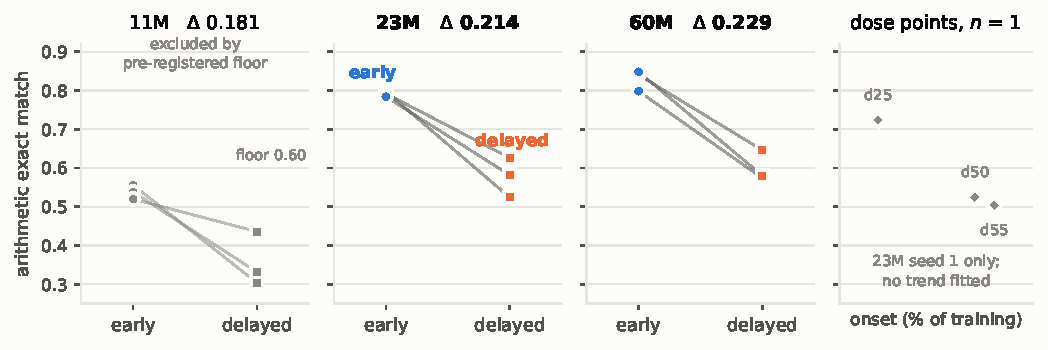
\includegraphics[width=\linewidth]{../logs/figures/fig1_detect.pdf}
\caption{Per-seed paired arithmetic endpoints at step 5000, early versus delayed exposure, one panel per model size, with the $n$~=~1 onset-dose points at right. The 11M panel is greyed: it falls below the pre-registered anchor floor and is excluded from the confirmatory comparison.}
\end{figure*}

\subsection{3.1 Delayed arithmetic exposure produces a persistent endpoint deficit}\label{delayed-arithmetic-exposure-produces-a-persistent-endpoint-deficit}

Every model in this section sees the same number of arithmetic tokens; the conditions
differ only in \emph{when} those tokens enter the stream. The delayed condition (d50) begins
arithmetic exposure at the midpoint of training, the early condition (d0) at step 0, and
both are read at step 5000 on the same 500 held-out problems. Because seeds are crossed (the same seed gives the same initialization in both conditions) the design-appropriate
statistic is the per-seed paired deficit, tested separately at each size and Holm-corrected
across the two confirmatory sizes.

\textbf{Table 1.} Arithmetic exact-match accuracy at step 5000, per seed and pooled.

\begin{table}[t]
\centering\small
\begin{tabular}{@{}
  >{\raggedright\arraybackslash}p{(\linewidth - 8\tabcolsep) * \real{0.2000}}
  >{\raggedleft\arraybackslash}p{(\linewidth - 8\tabcolsep) * \real{0.2000}}
  >{\raggedleft\arraybackslash}p{(\linewidth - 8\tabcolsep) * \real{0.2000}}
  >{\raggedleft\arraybackslash}p{(\linewidth - 8\tabcolsep) * \real{0.2000}}
  >{\raggedleft\arraybackslash}p{(\linewidth - 8\tabcolsep) * \real{0.2000}}@{}}
\toprule\noalign{}
\begin{minipage}[b]{\linewidth}\raggedright
size
\end{minipage} & \begin{minipage}[b]{\linewidth}\raggedleft
seed
\end{minipage} & \begin{minipage}[b]{\linewidth}\raggedleft
early (d0)
\end{minipage} & \begin{minipage}[b]{\linewidth}\raggedleft
delayed (d50)
\end{minipage} & \begin{minipage}[b]{\linewidth}\raggedleft
deficit
\end{minipage} \\
\midrule\noalign{}

23M & 1 & 0.798 & 0.524 & 0.274 \\
& 2 & 0.792 & 0.626 & 0.166 \\
& 3 & 0.784 & 0.582 & 0.202 \\
& \textbf{mean ± SD} & \textbf{0.791 ± 0.007} & \textbf{0.577 ± 0.051} & \textbf{0.214 ± 0.055} \\
60M & 1 & 0.798 & 0.574 & 0.224 \\
& 2 & 0.840 & 0.646 & 0.194 \\
& 3 & 0.848 & 0.580 & 0.268 \\
& \textbf{mean ± SD} & \textbf{0.829 ± 0.027} & \textbf{0.600 ± 0.040} & \textbf{0.229 ± 0.037} \\
\bottomrule
\end{tabular}
\end{table}


The deficit is present at every seed at both sizes: paired \emph{t}(2) = 6.74, \emph{p} = 0.0107 at
23M and \emph{t}(2) = 10.64, \emph{p} = 0.0044 at 60M, both surviving Holm correction within the
Detect family (adjusted 0.0107 and 0.0087; Hedges \emph{g} = 2.22 and 3.51). The pre-registered
Welch gate, which required a gap of at least 0.15, is cleared at both sizes (60M one-sided
\emph{p} = 0.0010). A model that receives its arithmetic exposure late does not catch up by the
end of training, despite having received all of it.

The deficit is of \textbf{similar magnitude at both sizes}: the 60M--23M difference is 0.015,
Welch \emph{p} = 0.72, MDE at 80 \% power \textbf{0.144}. That null constrains — it excludes any size
effect larger than about two-thirds of the deficit — but is not a claim that size is
irrelevant. §5.3 gives a structurally identical comparison carrying the opposite evidential
weight, because its MDE exceeds the entire range its outcome occupies; the two nulls are
best read as a pair.

\textbf{The deficit's severity is seed-variable, and the variability lives on the delayed side.}
The early anchor is tight (SD 0.007 at 23M) while the delayed endpoint is not (SD 0.051), so
per-seed deficits range 0.166--0.274 at 23M against a baseline that barely moves. Seed 1 is
deepest-hit on both readings and reproduces as such when retrained from scratch. Hence every
recovery result in §4 is an absolute endpoint beside its null rather than a percentage of a
seed-variable gap, which would be unstable by construction even when the effect is not.

\textbf{The 11M models are excluded by a pre-registered floor.} Their paired deficit is
nominally significant (0.181 ± 0.087, \emph{p} = 0.0345, \emph{g} = 1.19) and we report it, but the 11M
early anchor (0.538 ± 0.018) never plateaued and sits below the pre-registered 0.60 floor:
the comparison is between two under-trained models, so the difference cannot be attributed
to timing rather than capacity. This is a capacity boundary, not evidence against a critical
period at 11M.

Intermediate onsets (d25, d55, d75) were run at 23M seed 1 only, plotted without a fitted
trend; at \emph{n} = 1 they support no claim about the shape of the timing curve.

\subsection{\texorpdfstring{3.2 Long-distance \emph{wh}-licensing shows no detectable critical period}{3.2 Long-distance wh-licensing shows no detectable critical period}}\label{long-distance-wh-licensing-shows-no-detectable-critical-period}

The same design applied to long-distance \emph{wh}-licensing yields nothing. These are \textbf{five
different hypotheses about where an effect could hide, not five tests of one}; each carries
its own positive control or power statement, and that pairing is the argument, not the count.

\begin{enumerate}
\def\labelenumi{\arabic{enumi}.}
\tightlist
\item
  \textbf{Endpoint by delay} (\emph{n} = 3): no gap, against a delay-0 baseline that itself ranges
  0.520--0.586 over eight seeds (a spread exceeding any candidate effect) on the same
  harness that resolves arithmetic's 0.214.
\item
  \textbf{Acquisition dynamics}: Welch \emph{p} = 0.46, underpowered alone and carried by probe 3.
\item
  \textbf{Rate / bimodality}: a pre-registered compound gate over \textbf{72 runs} (24 seeds × 3
  sizes) returns DISCONFIRM: the mean rises monotonically with size (0.528 → 0.538 →
  0.552) but fails its floor at threshold 0.56 (top size 0.208 \textless{} 0.40) and its trend at
  0.57 (\emph{p} = 0.074), passing only at the permissive 0.55, and this powered test, sized in
  advance by simulation, is why long-distance syntax left the main grid.
\item
  \textbf{Representational probe}: delay-0 versus delay-50 \emph{p} = 0.48 \emph{while the same probe
  detects the structure at selectivity 0.60, p \textless{} 1e-8}: the positive control passes.
\item
  \textbf{Learning-rate budget} (hilr50, \emph{n} = 3): ΔLD = +0.011 ± 0.005, with Δlocal exceeding
  ΔLD at every seed and validation perplexity improving: a non-specific whole-model lift,
  not a rescue of the delayed skill.
\end{enumerate}

Probe 4 is load-bearing for a reason the others cannot supply: probes 1, 2, 3 and 5 ask
whether a critical period is visible \emph{in the behaviour that was acquired}, while probe 4 asks
whether the structure is encoded at all — and finds that it is, independent of when exposure
began. \textbf{The structure is learned; what is timing-invariant is the readout.} This null is
scoped to ≤ 60.3M parameters, the \textasciitilde10M-word BabyLM budget, and the continuation-scored
licensing-interaction metric.

\subsection{3.3 Skill dissociation}\label{skill-dissociation}

Under one design, one pipeline and matched total exposure, delayed exposure costs arithmetic
0.214 ± 0.055 and costs long-distance \emph{wh}-licensing nothing measurable across five probes.
That contrast is the paper's central detection-side result, and it inverts our
pre-registered prediction that syntax would show the \emph{stronger} critical period (§7.2).

\textbf{It must be stated in absolute terms, not as differential susceptibility, because the two
skills are not equally observable:}

\textbf{Table 2.} Why the dissociation is scoped.

\begin{table}[t]
\centering\small
\begin{tabular}{@{}
  >{\raggedright\arraybackslash}p{(\linewidth - 4\tabcolsep) * \real{0.3333}}
  >{\raggedleft\arraybackslash}p{(\linewidth - 4\tabcolsep) * \real{0.3333}}
  >{\raggedleft\arraybackslash}p{(\linewidth - 4\tabcolsep) * \real{0.3333}}@{}}
\toprule\noalign{}
\begin{minipage}[b]{\linewidth}\raggedright
\end{minipage} & \begin{minipage}[b]{\linewidth}\raggedleft
arithmetic
\end{minipage} & \begin{minipage}[b]{\linewidth}\raggedleft
syntax LD
\end{minipage} \\
\midrule\noalign{}

early-exposure anchor & 0.791 ± 0.007 & 0.528 (24 seeds) \\
chance floor & \textasciitilde0 (exact match) & 0.500 (by metric construction) \\
\textbf{headroom above floor} & \textbf{0.791} & \textbf{0.0283} \\
observed deficit & 0.214 (27.1 \% of headroom) & none detected \\
a proportionally matched deficit would be & --- & 0.0077 (0.49 seed-SD) \\
MDE at 80 \% power, \emph{n} = 3/group & --- & \textbf{0.0482} \\
\bottomrule
\end{tabular}
\end{table}


The long-distance design's MDE \textbf{exceeds its entire headroom by 1.7×}. A total collapse to
chance would be a change of 0.0283 — smaller than the smallest resolvable effect — and a
susceptibility proportionally identical to arithmetic's would require \emph{n} ≈ 67 per group. The
behavioural null therefore cannot, on its own, separate \emph{syntax is less susceptible} from
\emph{syntax had no room to show susceptibility}.

Only one probe rescues this. The learning-rate-budget null (probe 5) does \textbf{not}: it
establishes the ceiling is not an optimization-budget artifact, which \emph{preserves} the
dynamic-range limit rather than lifting it. The representational probe (probe 4) does — it
is the one readout not bounded by the 0.0283 headroom, it carries genuine dynamic range, and
it is flat across timing. Had delayed exposure damaged the underlying representation, that
probe had the range to register it and did not.

The differential-susceptibility reading remains open at a specific cost. Under the
mean-endpoint readout it is unmeasurable at this \emph{n}. Under a rate readout it is \textbf{un-run}:
the exceedance machinery was only pointed at the delay-0 question, and the seed inventory is
asymmetric (24 delay-0 seeds per size, 3 delayed at 23M alone). A rate-collapse test at 60M
(14 delayed seeds against the existing 24-seed baseline) would settle it; at 23M it needs 82
and is out of reach (§8).

Note what this is not. Our pre-registration anticipated a \emph{reopening}-side dissociation; what
the data support is a \emph{detection}-side one, since syntax never showed a deficit and no syntax
reopening was attempted. Superficially the same finding, not the same claim.

\section{§4 Reopen}\label{reopen}

\begin{figure*}[t]
\centering
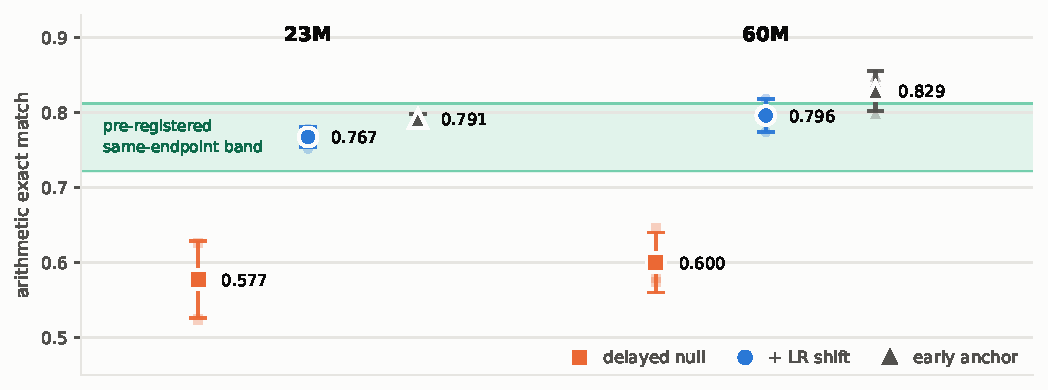
\includegraphics[width=\linewidth]{../logs/figures/fig2_reopen.pdf}
\caption{Absolute treated endpoints beside their untreated nulls and early-exposure anchors, with the pre-registered same-endpoint band shaded. Points are per-seed; bars are means $\pm$ SD across three seeds.}
\end{figure*}

\subsection{4.1 An LR-schedule shift restores the delayed endpoint}\label{an-lr-schedule-shift-restores-the-delayed-endpoint}

All intervention arms fork from a single saved checkpoint at step 2500 (identical weights,
optimizer state and step), so arms differ only in the intervention applied. The
\texttt{lr\_shift} arm restores the learning-rate schedule a delay-0 model would have been on when
delayed exposure begins, then anneals normally. Success was pre-registered as two conditions:
the treated endpoint must reach 90 \% of that run's \emph{own} early anchor, and general
capability must not degrade beyond a matched threshold.

\textbf{Table 3.} Endpoints at step 5000. The null is shown beside the treated arm throughout;
neither is collapsed into a ratio.

\begin{table}[t]
\centering\small
\begin{tabular}{@{}
  >{\raggedright\arraybackslash}p{(\linewidth - 12\tabcolsep) * \real{0.1429}}
  >{\raggedleft\arraybackslash}p{(\linewidth - 12\tabcolsep) * \real{0.1429}}
  >{\raggedleft\arraybackslash}p{(\linewidth - 12\tabcolsep) * \real{0.1429}}
  >{\raggedleft\arraybackslash}p{(\linewidth - 12\tabcolsep) * \real{0.1429}}
  >{\raggedleft\arraybackslash}p{(\linewidth - 12\tabcolsep) * \real{0.1429}}
  >{\raggedleft\arraybackslash}p{(\linewidth - 12\tabcolsep) * \real{0.1429}}
  >{\raggedleft\arraybackslash}p{(\linewidth - 12\tabcolsep) * \real{0.1429}}@{}}
\toprule\noalign{}
\begin{minipage}[b]{\linewidth}\raggedright
size
\end{minipage} & \begin{minipage}[b]{\linewidth}\raggedleft
treated (\texttt{lr\_shift})
\end{minipage} & \begin{minipage}[b]{\linewidth}\raggedleft
delayed null
\end{minipage} & \begin{minipage}[b]{\linewidth}\raggedleft
early anchor
\end{minipage} & \begin{minipage}[b]{\linewidth}\raggedleft
gate (0.90 × own d0)
\end{minipage} & \begin{minipage}[b]{\linewidth}\raggedleft
margin
\end{minipage} & \begin{minipage}[b]{\linewidth}\raggedleft
lift, \emph{p}
\end{minipage} \\
\midrule\noalign{}

23M & \textbf{0.767 ± 0.014} & 0.577 ± 0.051 & 0.791 ± 0.007 & 0.712 & +0.055 & 0.0065 \\
60M & \textbf{0.796 ± 0.022} & 0.600 ± 0.040 & 0.829 ± 0.027 & 0.746 & +0.050 & 0.0027 \\
\bottomrule
\end{tabular}
\end{table}


Per-seed treated endpoints are 0.752 / 0.778 / 0.772 at 23M and 0.796 / 0.818 / 0.774 at
60M. Every seed at both sizes clears its gate, and the per-seed lift over the matched null
survives Holm correction within the Reopen family (adjusted 0.0065 and 0.0054).

Two features of this table are more surprising than the recovery itself.

\textbf{The recovered endpoint is scale-invariant.} Both treated means fall inside the
pre-registered same-endpoint band {[}0.722, 0.812{]}, despite early anchors that differ by
0.038 and a 2.6× difference in parameters. Recovery converges on a level rather than
tracking capacity.

\textbf{The intervention collapses cross-seed variance.} The null's SD (0.051 at 23M, 0.040 at
60M) drops to the treated arm's (0.014, 0.022). The seed-variable severity documented in
§3.1 is a property of the \emph{untreated} delayed models; the intervention makes the outcome
both higher and more reproducible.

\subsection{4.2 The recovery does not come at the cost of general capability}\label{the-recovery-does-not-come-at-the-cost-of-general-capability}

Perplexity is reported as the three-number decomposition (early anchor \emph{a}, delayed null
\emph{b}, treated arm \emph{c}), because a single delta cannot distinguish a treated arm that
improved from a null that degraded.

At \textbf{23M there is no breach}: \emph{c} − \emph{b} = −0.889 / −0.204 / +0.193 across seeds, against a
pre-registered gate of +1.0 (seed 1: \emph{b} = 50.747, \emph{c} = 49.858, both from the canonical
\texttt{…seed1\_recheck} lineage). Two of three seeds improve.

At \textbf{60M the gate is tripped in all three seeds}: \emph{c} − \emph{b} = +1.670 ± 0.104 ppl, reported
as a trip and honoured as written. Two controls bound what it can mean. A no-op fork
reproduces the null on both perplexity and accuracy (Δppl −0.012, Δacc +0.011), so fork
mechanics contribute nothing. And at \textbf{matched learning rate} the treated arm \emph{leads} the
null by 2.478 ± 0.240 ppl — a lead larger than the breach — because it is read mid-anneal at
roughly six times the null's terminal learning rate, with ~4.15 ppl of annealing gain
unrealized. The breach persists only if the remaining anneal delivers less than 1.67 ppl of
that. Evidence leans toward near-full erasure, but the anneal slope is unmeasured, so we
quote \textbf{no point estimate}: the residual is bounded above by 1.67 ppl and a partly real cost
is not excluded. Extending the arm past step 5000 would collapse this bound (§8).

\subsection{4.3 The effect is specific to the delayed skill}\label{the-effect-is-specific-to-the-delayed-skill}

The same intervention applied to delayed \emph{syntax} models (all three seeds, matching the
arithmetic arm's depth) moves nothing: Δ local = −0.024 / −0.004 / +0.044 and Δ LD = −0.021 /
+0.007 / +0.015, sign-inconsistent around zero at every seed. A single-seed control could not
have distinguished ``no generic effect'' from ``an effect that landed near zero once'', which
is why it was run at the arm's own seed depth.

\subsection{4.4 Closure at this onset is largely a property of the schedule}\label{closure-at-this-onset-is-largely-a-property-of-the-schedule}

The remaining Tier-1 interventions were run at 23M seed 1 and are scored against the null's
cross-seed \textbf{range} {[}0.524, 0.626{]} rather than its mean, because a single seed landing
inside that range is indistinguishable from the null.

\begin{table}[t]
\centering\small
\begin{tabular}{@{}
  >{\raggedright\arraybackslash}p{(\linewidth - 4\tabcolsep) * \real{0.3333}}
  >{\raggedleft\arraybackslash}p{(\linewidth - 4\tabcolsep) * \real{0.3333}}
  >{\raggedright\arraybackslash}p{(\linewidth - 4\tabcolsep) * \real{0.3333}}@{}}
\toprule\noalign{}
\begin{minipage}[b]{\linewidth}\raggedright
arm (23M, seed 1)
\end{minipage} & \begin{minipage}[b]{\linewidth}\raggedleft
endpoint
\end{minipage} & \begin{minipage}[b]{\linewidth}\raggedright
verdict
\end{minipage} \\
\midrule\noalign{}

embedding reset & 0.586 & no detectable recovery (\emph{n} = 1) \\
reset + LR spike & 0.576 & no detectable recovery (\emph{n} = 1) \\
LR spike alone & 0.536 & no detectable recovery (\emph{n} = 1) \\
cram (concentrated re-exposure) & 0.574 & no detectable recovery (\emph{n} = 1) \\
\textbf{freeze} & \textbf{0.332} & \textbf{harmful}: below the entire null range \\
\bottomrule
\end{tabular}
\end{table}


Only freeze supports a directional statement at this depth. The others are \emph{not} evidence
that those interventions fail, but that one seed cannot separate them from a null whose own
spread is 0.10 wide. Embedding reset was our pre-registered favourite; §7.2 states that
prediction and its outcome.

The one arm extended to \emph{n} = 3 decides the mechanism. Concentrated re-exposure alone leaves
the endpoint at 0.574, at the null. Combined with the schedule shift it reaches
0.781 ± 0.031 — far above cram alone and indistinguishable from the shift by itself, with
per-seed differences of −0.006 / +0.016 / +0.032 straddling zero. (We report the signs
rather than the +0.014 mean: a near-zero mean with disagreeing signs is an absence of
effect, not a small effect obscured by pooling.)

So additional skill density on top of a restored schedule adds nothing, while a restored
schedule without additional density recovers the skill. \textbf{At this onset, what closes the
window is largely the optimizer's decayed learning-rate schedule rather than representations
that have hardened against revision.} The scope of that statement is d50, arithmetic, and
these two sizes; it is not a claim that entrenchment plays no role at other onsets.

The converse manipulation cannot be run cleanly. Imposing the late schedule segment on an
\emph{early} exposure window (one seed) collapses arithmetic from 0.778 to 0.142, the predicted
direction, but held-out perplexity degrades in step with it (69.2 to 87.9): the early window is
also where a randomly initialized model builds its base language model, so the manipulation
damages the substrate rather than isolating the skill window. The asymmetry is structural, not
statistical, because the forward arm intervenes on a model that has already built a healthy base
LM; additional seeds would replicate the confound rather than resolve it.


The schedule account predicts that if restoring the early segment merely raises accuracy, the
same shift should raise it on a model that was never delayed. Applied at 23M to the
early-exposure runs from their own step-2500 checkpoints, it does nothing: 0.783 ± 0.025
against an untreated anchor of 0.791 ± 0.007, a lift of −0.008 (per-seed −0.040 / +0.016 /
0.000), while the same intervention lifts the delayed runs +0.190. The whole reopening effect
requires the delayed exposure profile (alignment +0.198, positive at every seed, paired
\emph{t}(2) = 5.17, one-sided \emph{p} = 0.018). This rules out the reading that \texttt{lr\_shift} is simply a
better optimizer setting; it is not a second method confirming closure, which rests on cram.

A final arm belongs in the record without supporting a claim. The 11M \texttt{lr\_shift} arm passes
its gate (0.747 against 0.484), but degenerately: the gate is 90 \% of an anchor that failed
the §3.1 floor, and the arm \emph{exceeds its own early anchor} (0.538), indicating the 11M
anchor was learning-rate-starved. It enters only through its mechanism decomposition, where
the delayed lift of +0.389 splits into generic (+0.115) and exposure-alignment (+0.274)
components. That decomposition is exploratory and carries no headline; the 23M
discriminator above is its confirmatory-size counterpart, and its larger generic component
is what one expects if the 11M anchor was itself LR-starved.

\section{§5 Did the intervention repair the original circuit, or build a new one?}\label{did-the-intervention-repair-the-original-circuit-or-build-a-new-one}

Recovery tells us the skill came back; it does not tell us whether it came back \emph{in the same
machinery}. For each seed and size we compare a triad that shares an initialization: \textbf{A},
the early-exposure model; \textbf{B}, the delayed model; and \textbf{C}, the \texttt{lr\_shift}-recovered model
forked from B. Each model's arithmetic circuit is localized by mean-ablating attention heads
one at a time and recording exact-match damage. The decisive test is reciprocal: ablating
\textbf{A's} top heads inside \textbf{C} measures how much of A's circuit is still load-bearing in the
recovered model, and ablating \textbf{C's own} top heads inside C controls for C simply being
robust to any ablation. We report the transfer ratio (the damage A's heads do in C as a
fraction of the damage they do in A) where 1.0 means C inherited A's circuitry intact and 0
means A's heads are causally inert in C. One of the two size comparisons below is the
underpowered counterpart to §3.1's well-powered one; §5.3 makes that pairing explicit.

All numbers are computed on the single held-out problem set. An earlier version of this
analysis drew its eval items per-run, which overlapped training by 17--19 \% in four of the six
triads; all six were re-scored, the seed-1 triads reproduce exactly as a no-op control, and
the correction is reported in §2.4 because it changed a conclusion.

\subsection{5.1 Only one of four probes discriminates on this contrast}\label{only-one-of-four-probes-discriminates-on-this-contrast}

Which methods can tell the two outcomes apart \emph{at all} matters before reading anything off
the ablation numbers. Four were tried; three cannot:

\begin{itemize}
\tightlist
\item
  \textbf{Whole-layer mean-ablation saturates}: ablating any core layer drives accuracy to ~0 in
  every model, so localization is done at head granularity instead.
\item
  \textbf{Linear CKA} sits at 0.66--0.83 across all six triads regardless of what the causal test
  says. The triads share an initialization, so global geometry stays similar even where
  wiring differs; CKA scores the most reorganized triad at 0.658 and misses it.
\item
  \textbf{Single-head activation patching} is flat: restoration ratio spans 0.591--0.792 (SD 0.083)
  against ablation transfer's 0.187--0.868 (SD 0.265), uncorrelated (\emph{r} = 0.045, \emph{p} = 0.93;
  \emph{r} = −0.032 on corrected transfers, so the flatness is not a contamination artifact). The
  cause is a floor: single-head restoration is 0.05--0.15 in every model, so the ratio
  divides two small numbers. An earlier draft cited patching as corroboration on one seed;
  running all six withdrew that.
\item
  \textbf{Pruning-based localization} was pre-screened and rejected: mask overlap spans only 0.088,
  and its agreement with ablation \emph{flips sign} across the sparsity sweep. A method whose sign
  is a hyperparameter cannot adjudicate (Appendix A).
\end{itemize}

We therefore report this cluster as \textbf{single-method by demonstration}, not by assumption.
Three non-discriminating probes is itself the evidence for that label: the alternative,
citing agreement from a method never shown to resolve the contrast, is how the retracted
patching claim happened.

\subsection{5.2 Recovered circuits span a continuum, and it runs backwards at the shallow end}\label{recovered-circuits-span-a-continuum-and-it-runs-backwards-at-the-shallow-end}

\textbf{Table 4.} Reciprocal ablation transfer, ordered by deficit depth. Transfer = damage from
A's heads in C ÷ their damage in A. Control = damage from C's own heads ÷ damage from A's
heads in C, so a high control confirms C has a working circuit of its own.

\begin{table}[t]
\centering\small
\begin{tabular}{@{}
  >{\raggedright\arraybackslash}p{(\linewidth - 12\tabcolsep) * \real{0.1429}}
  >{\raggedleft\arraybackslash}p{(\linewidth - 12\tabcolsep) * \real{0.1429}}
  >{\raggedleft\arraybackslash}p{(\linewidth - 12\tabcolsep) * \real{0.1429}}
  >{\raggedleft\arraybackslash}p{(\linewidth - 12\tabcolsep) * \real{0.1429}}
  >{\raggedleft\arraybackslash}p{(\linewidth - 12\tabcolsep) * \real{0.1429}}
  >{\raggedleft\arraybackslash}p{(\linewidth - 12\tabcolsep) * \real{0.1429}}
  >{\raggedright\arraybackslash}p{(\linewidth - 12\tabcolsep) * \real{0.1429}}@{}}
\toprule\noalign{}
\begin{minipage}[b]{\linewidth}\raggedright
size
\end{minipage} & \begin{minipage}[b]{\linewidth}\raggedleft
seed
\end{minipage} & \begin{minipage}[b]{\linewidth}\raggedleft
deficit
\end{minipage} & \begin{minipage}[b]{\linewidth}\raggedleft
transfer
\end{minipage} & \begin{minipage}[b]{\linewidth}\raggedleft
control
\end{minipage} & \begin{minipage}[b]{\linewidth}\raggedleft
Jaccard(A, C)
\end{minipage} & \begin{minipage}[b]{\linewidth}\raggedright
pre-registered verdict
\end{minipage} \\
\midrule\noalign{}

23M & 2 & 0.182 & 0.659 & 1.50 & 0.00 & mixed / partial \\
60M & 2 & 0.202 & 0.404 & 2.43 & 0.00 & mixed / partial \\
23M & 3 & 0.210 & 0.868 & 1.16 & 0.20 & mixed / partial \\
60M & 1 & 0.224 & 0.445 & 2.18 & 0.09 & mixed / partial \\
60M & 3 & 0.260 & 0.201 & 5.13 & 0.00 & new circuit \\
23M & 1 & 0.292 & 0.187 & 5.36 & 0.00 & new circuit \\
\bottomrule
\end{tabular}
\end{table}


Recovered models do not behave alike. They span a continuum from near-complete transfer of
the original circuit to full reorganization. At one end (23M seed 3) the recovered model
inherits 87 \% of the damage A's circuit takes, and its own top heads are barely more damaging
than A's: the original machinery is still carrying the skill. At the other (23M seed 1, 60M
seed 3) A's heads are close to inert in C while C's own heads are five times more damaging:
the skill returned in different machinery. \textbf{Every 60M triad sits at or below 0.445}, so at
the larger size reorganization is what we observe at every seed.

We report this axis continuously and assign no categorical verdict. Our implementation would
have labelled a triad \emph{repaired} only on a conjunction of high transfer \emph{and} high
top-head-set overlap; the overlap condition is never met here (maximum 0.20), so the label
was unreachable. It was an implementation default rather than a registered criterion, and
relabelling now would be choosing a decision rule after seeing the number it decides
(Appendix B). The mismatch is the methodological point: a recovered model's head set can
overlap its baseline's almost not at all while the baseline's heads remain causally
load-bearing — near-zero overlap at transfer 0.868. \textbf{Set overlap and causal overlap are
different measurements}, and only the second answers the question; that is the case for
reciprocal ablation over any similarity-of-components measure, and the same failure that
makes CKA useless here.

The ordering suggests deficit depth grades this outcome, but the evidence does not survive
its own robustness check: Spearman ρ = −0.714, exact permutation \emph{p} = 0.0681, and
leave-one-out is fragile, with four of six deletions pushing \emph{p} above 0.05. The direction
persists but is not resolvable at \emph{n} = 6. More triads are the only thing that would settle
it, and this is the one place where additional runs would still move a headline.

One pair runs backwards, and it is the best-measured comparison in the table. At 23M, seeds
2 and 3 have nearly the same deficit (0.182 vs 0.210), yet the \emph{deeper} one shows \emph{more}
repair (0.868 vs 0.659), with non-overlapping bootstrap intervals {[}0.832, 0.903{]} against
{[}0.611, 0.708{]}. Those intervals reflect eval-item variance at one model per point, so they
say the two measurements differ, not that two populations do — but within the shallow-deficit
regime the severity ordering inverts. Whatever grades circuit identity is not deficit depth
alone.

\subsection{5.3 On size, this design is underpowered, unlike the one in §3.1}\label{on-size-this-design-is-underpowered-unlike-the-one-in-3.1}

Transfer averages 0.571 ± 0.349 at 23M and 0.350 ± 0.131 at 60M (Welch \emph{p} = 0.39). \textbf{That
non-significance means nothing here.} The minimum detectable effect at 80 \% power is 0.809,
against an outcome span of only 0.681 across all six triads: no difference this design could
have produced would have been detected. The question is \emph{untested}, not answered, and it is
no longer unidentifiable, since the corrected deficit ranges at the two sizes overlap, so
size is separable from deficit depth in a way it was not before the contamination fix.

Set this beside §3.1's structurally identical comparison (same \emph{n} = 3 per group, same Welch
test, same two sizes, also non-significant), which carries opposite weight: there the MDE
(0.144) sits below the deficit being asked about (0.21), so the null genuinely excludes a
large size effect, while here it exceeds the entire measured range. Non-significance is read
off the minimum detectable effect, never off the \emph{p}.

What the size axis does show is \textbf{variance}: the 60M transfers are tightly clustered
(SD 0.131) where the 23M ones are not (SD 0.349), a 2.7× ratio mirroring §4's finding that the
intervention collapses cross-seed variance. Suggestive only — one comparison at \emph{n} = 3 per
group on an observational rather than manipulated factor.

\subsection{5.4 What these results do not speak to}\label{what-these-results-do-not-speak-to}

Our third pre-registered prediction linked circuit identity to the reset intervention: if
reset were the winning intervention, we expected it to build a new circuit. Reset never
produced recovery (§4.4), so the antecedent never occurred and the prediction was never
entered. The models diagnosed here are \texttt{lr\_shift}-recovered, which that prediction did not
cover; §7.2 states this rather than letting the section read as an answer to it.

Three further quantities appear in our released logs and support nothing. The within-60M
Spearman is mechanical at \emph{n} = 3. An extrapolation from the 23M triads onto the 60M points
was built before the contamination correction and no longer fits (residuals −0.30, −0.15,
−0.20). Numbers from the causal-tracing and pruning scripts were computed on the contaminated
draws and were never re-run, since neither supports a surviving claim. Circuit redundancy and
sufficiency are likewise untested here: the retracted patching analysis was the only probe
that addressed them.

\section{§6 A secondary probe: agreement attraction across scale}\label{a-secondary-probe-agreement-attraction-across-scale}

These models support one question the critical-period design did not set out to ask.
Subject--verb agreement is acquired almost perfectly (0.98 on controlled items) yet fails when
a number-mismatching noun intervenes. A fully-crossed design, in which the verb-form frequency
prior cancels \emph{exactly}, separates \textbf{attraction} (an intervening noun mismatching the head in
number) from \textbf{complexity} (any intervening material).

\textbf{Attraction is real, large, and dominant.} At 23.2M it costs +0.303 ± 0.064
(\emph{p} = 8.6e-05) against complexity's +0.143 ± 0.035, in both number directions and both frame
types. A unigram-frequency control returns exactly 0.000 by construction, so it cannot be a
verb-form prior. Attraction exceeds complexity at every size and is positive in \textbf{81 of 81
models} across two mixtures: 72 syntax-enriched (3 sizes × 24 seeds) and 9 arithmetic-enriched.

\textbf{Whether these models are anti-syntactic is scale-dependent.} Mismatch accuracy is 0.405 at
11.5M (below chance, \emph{p} \textless{} 0.001), 0.511 at 23.2M (at chance, \emph{p} = 0.435), and 0.610 at 60.3M
(above chance, \emph{p} \textless{} 0.001): below-chance agreement occurs only at the smallest size.

\textbf{Attraction declines with scale; whether it dissociates from complexity depends on the
mixture.} In the syntax-enriched mixture attraction falls \textbf{−0.316 per decade of
parameters} (\emph{r} = −0.803, \emph{p} = 2.3e-17, \emph{n} = 72), from +0.430 to +0.201, while complexity is
\textbf{flat} (+0.016/decade, \emph{p} = 0.43). The second mixture reproduces the attraction half in
direction and magnitude, \textbf{−0.207/decade}, stable at −0.21 to −0.24 under every estimator
but at \textbf{estimator-dependent significance (\emph{p} = 0.033 OLS, 0.073 robust SE)} on an
unbalanced (3, 3, 8) design whose leverage sits on the under-sampled small end. It does
\textbf{not} reproduce the dissociation: complexity falls there too, and the paired within-model
contrast is flat (−0.095, \emph{p} = 0.36) against −0.333 (\emph{p} = 3.8e-11) in the syntax mixture —
the one part not estimator-fragile. A cross-mixture divergence at 60.3M \textbf{does not survive
replication} at \emph{n} = 8 (+0.065, \emph{p} = 0.091, halved from +0.133) and \textbf{is not excluded}: the
95 \% CI still contains the original effect. An English-exposure explanation is excluded
separately, since exposure is constant across sizes by design.

\textbf{Attraction may also decline \emph{within} a single run}, +0.392 → +0.303 between steps 2500 and 5000 (paired, \emph{n} = 6): marginal at \emph{p} = 0.053 with 53 \% power and an MDE of 0.125, so we report it as suggestive only; Appendix C gives the power calculation.

\textbf{The standard metric gets this wrong at every scale, in three ways.} Uncontrolled
BLiMP-style items report below-chance behaviour at all three sizes, true only at the
smallest; the frequency-controlled metric locates it correctly; and only the crossed design
separates attraction from complexity. Three metrics, three conclusions, same models.
Relatedly, pooling all 72 models into one attraction estimate averages across a
size-dependent effect and yields a number describing no size.

This is also why the skill sits here rather than §3: agreement saturates by step 2500 and
its supporting structure appears in ~39 \% of the corpus against \emph{wh}-extraction's 1.5 \%, so
it cannot meaningfully be withheld. Being \emph{learnable enough to measure} and being
\emph{delayable} are different properties, and this design needs both.

\section{§7 Discussion}\label{discussion}

\subsection{7.1 Two timing results at different levels}\label{two-timing-results-at-different-levels}

Two findings about timing, at different levels. \emph{Which} skills a late start damages is
skill-specific: arithmetic pays a persistent cost, long-distance \emph{wh}-licensing pays nothing
measurable. And where damage occurs it is carried by the optimizer's learning-rate schedule
rather than by hardened representations — restoring the schedule restores the skill, adding
skill data without it does not. A late start hurts some skills and not others; when it
hurts, what has closed is the model's step size, not its mind.

The second finding survives the obvious deflationary reading. Applied at 23M to models that
were never delayed, the same shift does nothing (−0.008, against +0.190 on the delayed runs),
so recovery is specific to the delayed exposure profile, not a generic optimizer gain
(§4.4) — which rules out one alternative reading without being a second method confirming
closure, and closure still rests on the cram contrast alone.

\subsection{7.2 The three pre-registered predictions}\label{the-three-pre-registered-predictions}

\textbf{\#1 (syntax would show the \emph{stronger} critical period) was inverted.} We reasoned that
long-distance dependencies, scaffolded by earlier-acquired structure, would be more fragile
to a late start; arithmetic carries the effect instead. This inversion is the origin of
§3.3's dissociation, not an incidental miss.

\textbf{\#2 (embedding reset would be the most effective intervention) was not borne out.} Reset
landed at 0.586 against a null spanning {[}0.524, 0.626{]}, and the learning-rate shift was the
only arm to clear the gate. At a single seed this is a statement about what we could detect,
not a demonstration that reset fails. The prediction's second half (largest forgetting risk)
was also not observed.

\textbf{\#3 (a reset-driven recovery would build new circuitry) was never testable}, being
conditional on reset winning. §5 diagnoses models recovered by the learning-rate shift, which
\#3 did not cover; those results confirm and disconfirm nothing about it. We say so because §5
is where a reader holding our pre-registration will look for the answer.

\subsection{7.3 What the mechanism result does not say}\label{what-the-mechanism-result-does-not-say}

Schedule-driven closure is demonstrated at one onset, for one skill, at two sizes. It is not
a claim that representational entrenchment plays no role in critical periods generally, nor
at later onsets in this setup. Our intermediate-onset runs are single-seed and say nothing
about the shape of the timing curve.

\begin{center}\rule{0.5\linewidth}{0.5pt}\end{center}

\section{§8 Limitations}\label{limitations}

Five experiments would move a label, named with their costs rather than gestured at.
\textbf{The dissociation's stronger reading is un-run, not unknowable}: whether syntax is genuinely
\emph{less susceptible} rather than lacking headroom is decidable by a rate-collapse test at 60M,
14 delayed seeds against our existing 24-seed baseline (Appendix C) — the cheapest
outstanding experiment and the only one that can promote the dissociation past its scope.
\textbf{The 60M perplexity cost is bounded, not estimated}: extending the treated arm past step
5,000 to complete annealing would convert the 1.67 ppl upper bound into a point estimate.
\textbf{The circuit-identity gradient is unresolved at \emph{n} = 6}: more triads are the only thing that
would settle whether deficit depth grades identity, since four of six leave-one-out
deletions break significance. \textbf{The circuit results are single-method by demonstration}:
joint head-group patching, if shown to have dynamic range on this contrast, would drop the
annotation. \textbf{One agreement-attraction slope is estimator-dependent}: three or more seeds at
the smallest size would rebalance the leverage behind it.

Beyond these: one corpus, one tokenizer, one language, a maximum of 60.3M parameters, and a
single delay onset carrying the reopening result. Five of six intervention arms are single
seed. The smallest size is excluded by a floor rather than solved.

\begin{center}\rule{0.5\linewidth}{0.5pt}\end{center}

\section{§9 Conclusion}\label{conclusion}

Timing of exposure matters in these models, but not uniformly and not for the reason we
expected. Delayed arithmetic exposure leaves a deficit that further training does not close;
delayed long-distance \emph{wh}-licensing leaves nothing we can detect, which inverts our
prediction and which we state in absolute terms because the two skills are not equally
observable. Where the deficit exists it reopens, and it reopens when the learning-rate
schedule is restored rather than when the missed data is concentrated, so what closes at
this onset behaves like a property of the optimizer rather than of entrenched representation.
Whether the skill contrast reflects genuine differential susceptibility remains open, and we
have named the fourteen-seed experiment that would decide it.

\begin{center}\rule{0.5\linewidth}{0.5pt}\end{center}

\textbf{Relation to prior work.} Critical periods are established in
development and, for vision models, in Achille et al.'s demonstration that an early deficit
leaves a permanent gap \citep{achille-etal-2019}; we manipulate \emph{when} a skill's data arrives
rather than its quality, holding total exposure fixed. The nearest explanation of our
reopening result is plasticity loss and warm starting
\citep{ash-adams-2020,dohare-etal-2024,lyle-etal-2023}. The difference is specific: those
settings involve a distribution shift, a restart, or a sequence of distinct tasks and
recover plasticity by perturbing \emph{weights}, whereas our models train once on a stationary
mixture whose only manipulated variable is a skill's onset step, and the intervention that
recovers the skill changes no weights at all — while weight resetting, the standard
plasticity remedy, produced no detectable recovery (\emph{n} = 1, §7.2). The mechanisms may yet be
one thing seen from two directions; recovery here needs no weight perturbation. The result
is also distinct from grokking \citep{power-etal-2022}, where data is fixed and
generalization is sudden. Our circuit diagnosis sits in the causal-ablation and
activation-patching tradition \citep{elhage-etal-2021,wang-etal-2023,meng-etal-2022} alongside
representational similarity \citep{kornblith-etal-2019}; §5.1's negative methodological
result is that three of those four probes do not discriminate here.

\bibliography{references}

\appendix
\section{Appendix A. Pruning-based localization: the pre-screen that rejected it}\label{appendix-a.-pruning-based-localization-the-pre-screen-that-rejected-it}

Pruning was rejected by a pre-screen fixed in advance
(\texttt{notes/week8-pruning-feasibility-prereg.md}), before the full tool was built. We report it
because the rejection came within one hyperparameter of looking like a confirmation.

\textbf{Method.} Learned binary gates over heads and MLPs, objective = arithmetic answer-span
cross-entropy + λ‖g‖₁, binarized at 0.5; cross-model readout IoU(mask(A), mask(C)).

\textbf{Four gates, fixed in advance; two failed.}

\begin{table}[t]
\centering\small
\begin{tabular}{@{}
  >{\raggedright\arraybackslash}p{(\linewidth - 4\tabcolsep) * \real{0.3333}}
  >{\raggedright\arraybackslash}p{(\linewidth - 4\tabcolsep) * \real{0.3333}}
  >{\raggedright\arraybackslash}p{(\linewidth - 4\tabcolsep) * \real{0.3333}}@{}}
\toprule\noalign{}
\begin{minipage}[b]{\linewidth}\raggedright
gate
\end{minipage} & \begin{minipage}[b]{\linewidth}\raggedright
threshold
\end{minipage} & \begin{minipage}[b]{\linewidth}\raggedright
result
\end{minipage} \\
\midrule\noalign{}

1. reproducibility & IoU(A, A′) ≥ 0.70 on two independent fits & \textbf{PASS}: 1.000, the two fits give the identical mask \\
2. dynamic range & spread of IoU(A, C) ≥ 0.20 across seeds & \textbf{FAIL}: 0.088, all three inside one 0.10-wide band \\
3. ordering & seed 1 (most reorganized by ablation) lowest & \textbf{FAIL}: seed 3 is lowest at 0.425; seed 1 is middle \\
4. functional validity & mask retains ≥ 0.80 of accuracy & \textbf{PASS}: 0.80--0.94 on \textasciitilde30/54 components; complement → 0.000 \\
\bottomrule
\end{tabular}
\end{table}


The metric is real — reproducible, and the mask genuinely is a sufficient arithmetic
subnetwork — but it does not track circuit identity: A and C overlap about the same amount
whether or not C rebuilt.

\textbf{The sparsity sweep, run to pre-empt ``you picked the wrong λ'', found worse than
insensitivity.}

\begin{table}[t]
\centering\small
\begin{tabular}{@{}
  >{\raggedleft\arraybackslash}p{(\linewidth - 10\tabcolsep) * \real{0.1667}}
  >{\raggedright\arraybackslash}p{(\linewidth - 10\tabcolsep) * \real{0.1667}}
  >{\raggedleft\arraybackslash}p{(\linewidth - 10\tabcolsep) * \real{0.1667}}
  >{\raggedleft\arraybackslash}p{(\linewidth - 10\tabcolsep) * \real{0.1667}}
  >{\raggedright\arraybackslash}p{(\linewidth - 10\tabcolsep) * \real{0.1667}}
  >{\raggedright\arraybackslash}p{(\linewidth - 10\tabcolsep) * \real{0.1667}}@{}}
\toprule\noalign{}
\begin{minipage}[b]{\linewidth}\raggedleft
λ
\end{minipage} & \begin{minipage}[b]{\linewidth}\raggedright
IoU seed 1 / 2 / 3
\end{minipage} & \begin{minipage}[b]{\linewidth}\raggedleft
spread
\end{minipage} & \begin{minipage}[b]{\linewidth}\raggedleft
\emph{r} vs ablation transfer
\end{minipage} & \begin{minipage}[b]{\linewidth}\raggedright
mask retains A's accuracy
\end{minipage} & \begin{minipage}[b]{\linewidth}\raggedright
gate 4
\end{minipage} \\
\midrule\noalign{}

0.01 & 0.609 / 0.511 / 0.523 & 0.098 & \textbf{−0.944} & 0.89 / 0.99 / 0.94 & pass \\
0.03 & 0.442 / 0.513 / 0.425 & 0.088 & \textbf{+0.118} & 0.80 / 0.94 / 0.81 & pass \\
0.06 & 0.333 / 0.529 / 0.472 & 0.196 & \textbf{+0.872} & 0.67 / 0.70 / 0.83 & \textbf{FAIL} \\
\bottomrule
\end{tabular}
\end{table}


Seed 1's overlap moves monotonically from \emph{highest} to \emph{middle} to \emph{lowest} as the mask
tightens: \textbf{the sign of the method's answer is set by a hyperparameter, not by the models}.
And the λ that agrees with the primary readout (\emph{r} = +0.872) is exactly the λ at which the
mask stops being a valid circuit — retention 0.67 / 0.70, below the pre-registered 0.80 bar.
Run at λ = 0.06 alone, this pilot would have reported ``pruning independently confirms
reorganization'' — the same shape as the retracted single-head patching result (§5.1), and
wrong for the same reason: a secondary method cited as corroboration without being shown to
discriminate across the contrast set. Hence §5's claims are single-method by demonstration.

\begin{center}\rule{0.5\linewidth}{0.5pt}\end{center}

\section{Appendix B: Provenance of the circuit-identity classifier's thresholds}\label{appendix-b-provenance-of-the-circuit-identity-classifiers-thresholds}

§5.2 reports the transfer axis continuously and assigns no categorical verdict. Our
implementation classified a triad as \emph{repaired} when transfer ≥ 0.6 \textbf{and} IoU of the two
models' top-head sets ≥ 0.4. The second conjunct is never satisfied here (maximum 0.20
across six triads), so the repair label was unreachable. Four facts about that rule
(checked 2026-08-05): it was \textbf{not pre-registered} — the genuine pre-registration
(\texttt{notes/week8-diagnosis-seed-scope.md}) fixes seed scope and diagnostics but specifies no
thresholds and no overlap criterion; it is a \textbf{code-level default}
(\texttt{scripts/week8\_circuit\_identity.py:276-278}); it \textbf{contradicts its own docstring
asymmetrically} (``Primary = transfer\_ratio \ldots{} Jaccard \emph{corroborates}'', yet overlap is a
hard conjunct on the repair branch only); and it was \textbf{contradicted by the first triad that
tested it and then formally demoted without the code changing}
(\texttt{notes/week8-60M-seed2-prereg.md}: ``it did NOT discriminate at 23M: seed 2 had Jaccard
0.09 \emph{with} transfer 0.71''). So ``no triad was classified as repair'' describes a stale
conjunct, not the models.

We did not simply relabel: dropping the conjunct would move the highest-transfer triad
(23M seed 3, transfer 0.868) into \emph{repair}, which is choosing a decision rule after seeing
the number it decides. The continuous axis assumes neither rule, and the verdict column
stays in Table 4 so the absent repair row is visible. Measurements are untouched
throughout; only the labelling was in question. The generalizable point: a decision
recorded in a pre-registration does not propagate itself into code.

\begin{center}\rule{0.5\linewidth}{0.5pt}\end{center}

\section{Appendix C: Settings and supporting counts}\label{appendix-c-settings-and-supporting-counts}

\subsection{C.1 Architecture and optimizer settings}\label{c.1-architecture-and-optimizer-settings}

Context length 512; rotary positions (θ = 10,000); pre-norm; GELU. Attention is
\texttt{F.scaled\_dot\_product\_attention} (FlashAttention-2 kernels). Training uses bf16 autocast,
micro-batches of 8 × 512 tokens with 4 gradient accumulation steps, and AdamW
(β = 0.9/0.95, weight decay 0.1, gradient clipping 1.0). \texttt{torch.compile} was
\textbf{disabled for every run}. Checkpoint spacing (100 steps for 23M arithmetic, 1,250 at
11M and 60M, 2,500 for the size sweep) sets only how finely a trajectory can be re-read;
delay and intervention triggers fire on exact step count.

\subsection{C.2 Parameter counts and the embedding share}\label{c.2-parameter-counts-and-the-embedding-share}

Recomputed from the step-5000 checkpoint state dicts (\texttt{scripts/param\_counts.py}), which
asserts each checkpoint's stored \texttt{model\_config} matches its weights.

\begin{table}[t]
\centering\small
\begin{tabular}{@{}
  >{\raggedright\arraybackslash}p{(\linewidth - 16\tabcolsep) * \real{0.1111}}
  >{\raggedleft\arraybackslash}p{(\linewidth - 16\tabcolsep) * \real{0.1111}}
  >{\raggedleft\arraybackslash}p{(\linewidth - 16\tabcolsep) * \real{0.1111}}
  >{\raggedleft\arraybackslash}p{(\linewidth - 16\tabcolsep) * \real{0.1111}}
  >{\raggedleft\arraybackslash}p{(\linewidth - 16\tabcolsep) * \real{0.1111}}
  >{\raggedleft\arraybackslash}p{(\linewidth - 16\tabcolsep) * \real{0.1111}}
  >{\raggedleft\arraybackslash}p{(\linewidth - 16\tabcolsep) * \real{0.1111}}
  >{\raggedleft\arraybackslash}p{(\linewidth - 16\tabcolsep) * \real{0.1111}}
  >{\raggedleft\arraybackslash}p{(\linewidth - 16\tabcolsep) * \real{0.1111}}@{}}
\toprule\noalign{}
\begin{minipage}[b]{\linewidth}\raggedright
tag
\end{minipage} & \begin{minipage}[b]{\linewidth}\raggedleft
layers
\end{minipage} & \begin{minipage}[b]{\linewidth}\raggedleft
heads
\end{minipage} & \begin{minipage}[b]{\linewidth}\raggedleft
width
\end{minipage} & \begin{minipage}[b]{\linewidth}\raggedleft
vocab
\end{minipage} & \begin{minipage}[b]{\linewidth}\raggedleft
total
\end{minipage} & \begin{minipage}[b]{\linewidth}\raggedleft
non-embedding
\end{minipage} & \begin{minipage}[b]{\linewidth}\raggedleft
embed+head
\end{minipage} & \begin{minipage}[b]{\linewidth}\raggedleft
embed share
\end{minipage} \\
\midrule\noalign{}

11M & 4 & 8 & 256 & 16,384 & 11,536,640 & 3,148,032 & 8,388,608 & 72.7 \% \\
23M & 6 & 8 & 384 & 16,384 & 23,204,736 & 10,621,824 & 12,582,912 & 54.2 \% \\
60M & 8 & 10 & 640 & 16,384 & 60,304,000 & 39,332,480 & 20,971,520 & 34.8 \% \\
\bottomrule
\end{tabular}
\end{table}




\subsection{C.3 Why the three pre-registered analyses are not estimable}\label{c.3-why-the-three-pre-registered-analyses-are-not-estimable}

\textbf{Mixed-effects \texttt{accuracy\ \textasciitilde{}\ delay\ ×\ model\_size}}: after the floor exclusion,
twelve observations, one per seed × cell, so no within-cell replication for a random
effect. \textbf{\texttt{recovery\%\ \textasciitilde{}\ intervention\ ×\ skill\ ×\ delay\_onset}}: the response divides
by the seed-variable delayed null, two of three factors are constants, and only one
intervention arm reaches \emph{n} = 3. \textbf{\texttt{circuit\_overlap\ \textasciitilde{}\ intervention\ ×\ skill}}:
both factors are constants.

\subsection{C.4 The attraction trajectory: power}\label{c.4-the-attraction-trajectory-power}

Between steps 2500 and 5000 the isolated attraction cost falls +0.392 → +0.303 (paired,
\emph{n} = 6 at 23.2M, 5/6 seeds), marginal at \emph{p} = 0.053, with \textbf{53 \% power and an MDE of 0.125}:
roughly ten seeds would decide it. The mismatch cell improves significantly over the same
interval (+0.070, \emph{p} = 0.041), the non-marginal part. Per-seed trajectories are unavailable:
step-2500 evaluations were recorded only as a paired aggregate.

\subsection{C.5 Seed counts for the outstanding tests}\label{c.5-seed-counts-for-the-outstanding-tests}

Counts for the §8 rate-collapse test, assuming delay \emph{eliminates} the high-acquisition mode;
if it merely \emph{halves} the mode, the requirement rises to 59 per group at 60M and 203 at 23M.

\begin{table}[h]
\centering\small
\begin{tabular}{@{}lrl@{}}
\toprule\noalign{}
test & seeds needed & status \\
\midrule\noalign{}

60M @ 0.5593 & \textbf{14} & no delayed 60M seeds exist yet \\
60M @ 0.55 (permissive) & 6 & --- \\
23M @ 0.5593 & 82 & out of reach \\
23M @ 0.55 (permissive) & 18 & current \emph{n} = 3 gives \emph{p} = 0.786 \\
\bottomrule
\end{tabular}
\end{table}


\begin{center}\rule{0.5\linewidth}{0.5pt}\end{center}

\end{document}
